\documentclass[twoside]{book}

% Packages required by doxygen
\usepackage{fixltx2e}
\usepackage{calc}
\usepackage{doxygen}
\usepackage[export]{adjustbox} % also loads graphicx
\usepackage{graphicx}
\usepackage[utf8]{inputenc}
\usepackage{makeidx}
\usepackage{multicol}
\usepackage{multirow}
\PassOptionsToPackage{warn}{textcomp}
\usepackage{textcomp}
\usepackage[nointegrals]{wasysym}
\usepackage[table]{xcolor}

% NLS support packages
\usepackage[french]{babel}

% Font selection
\usepackage[T1]{fontenc}
\usepackage[scaled=.90]{helvet}
\usepackage{courier}
\usepackage{amssymb}
\usepackage{sectsty}
\renewcommand{\familydefault}{\sfdefault}
\allsectionsfont{%
  \fontseries{bc}\selectfont%
  \color{darkgray}%
}
\renewcommand{\DoxyLabelFont}{%
  \fontseries{bc}\selectfont%
  \color{darkgray}%
}
\newcommand{\+}{\discretionary{\mbox{\scriptsize$\hookleftarrow$}}{}{}}

% Page & text layout
\usepackage{geometry}
\geometry{%
  a4paper,%
  top=2.5cm,%
  bottom=2.5cm,%
  left=2.5cm,%
  right=2.5cm%
}
\tolerance=750
\hfuzz=15pt
\hbadness=750
\setlength{\emergencystretch}{15pt}
\setlength{\parindent}{0cm}
\setlength{\parskip}{3ex plus 2ex minus 2ex}
\makeatletter
\renewcommand{\paragraph}{%
  \@startsection{paragraph}{4}{0ex}{-1.0ex}{1.0ex}{%
    \normalfont\normalsize\bfseries\SS@parafont%
  }%
}
\renewcommand{\subparagraph}{%
  \@startsection{subparagraph}{5}{0ex}{-1.0ex}{1.0ex}{%
    \normalfont\normalsize\bfseries\SS@subparafont%
  }%
}
\makeatother

% Headers & footers
\usepackage{fancyhdr}
\pagestyle{fancyplain}
\fancyhead[LE]{\fancyplain{}{\bfseries\thepage}}
\fancyhead[CE]{\fancyplain{}{}}
\fancyhead[RE]{\fancyplain{}{\bfseries\leftmark}}
\fancyhead[LO]{\fancyplain{}{\bfseries\rightmark}}
\fancyhead[CO]{\fancyplain{}{}}
\fancyhead[RO]{\fancyplain{}{\bfseries\thepage}}
\fancyfoot[LE]{\fancyplain{}{}}
\fancyfoot[CE]{\fancyplain{}{}}
\fancyfoot[RE]{\fancyplain{}{\bfseries\scriptsize Généré par Doxygen }}
\fancyfoot[LO]{\fancyplain{}{\bfseries\scriptsize Généré par Doxygen }}
\fancyfoot[CO]{\fancyplain{}{}}
\fancyfoot[RO]{\fancyplain{}{}}
\renewcommand{\footrulewidth}{0.4pt}
\renewcommand{\chaptermark}[1]{%
  \markboth{#1}{}%
}
\renewcommand{\sectionmark}[1]{%
  \markright{\thesection\ #1}%
}

% Indices & bibliography
\usepackage{natbib}
\usepackage[titles]{tocloft}
\setcounter{tocdepth}{3}
\setcounter{secnumdepth}{5}
\makeindex

% Hyperlinks (required, but should be loaded last)
\usepackage{ifpdf}
\ifpdf
  \usepackage[pdftex,pagebackref=true]{hyperref}
\else
  \usepackage[ps2pdf,pagebackref=true]{hyperref}
\fi
\hypersetup{%
  colorlinks=true,%
  linkcolor=blue,%
  citecolor=blue,%
  unicode%
}

% Custom commands
\newcommand{\clearemptydoublepage}{%
  \newpage{\pagestyle{empty}\cleardoublepage}%
}

\usepackage{caption}
\captionsetup{labelsep=space,justification=centering,font={bf},singlelinecheck=off,skip=4pt,position=top}

%===== C O N T E N T S =====

\begin{document}

% Titlepage & ToC
\hypersetup{pageanchor=false,
             bookmarksnumbered=true,
             pdfencoding=unicode
            }
\pagenumbering{alph}
\begin{titlepage}
\vspace*{7cm}
\begin{center}%
{\Large Argument Parser \\[1ex]\large 1.\+0.\+0 }\\
\vspace*{1cm}
{\large Généré par Doxygen 1.8.12}\\
\end{center}
\end{titlepage}
\clearemptydoublepage
\pagenumbering{roman}
\tableofcontents
\clearemptydoublepage
\pagenumbering{arabic}
\hypersetup{pageanchor=true}

%--- Begin generated contents ---
\chapter{Index des fichiers}
\section{Liste des fichiers}
Liste de tous les fichiers avec une brève description \+:\begin{DoxyCompactList}
\item\contentsline{section}{include/\hyperlink{arguparser_8h}{arguparser.\+h} }{\pageref{arguparser_8h}}{}
\item\contentsline{section}{include/\hyperlink{numbers_8h}{numbers.\+h} \\*Toutes les fonctions en relation avec des nombres }{\pageref{numbers_8h}}{}
\item\contentsline{section}{src/numbers/\hyperlink{validation_8c}{validation.\+c} \\*Déclaration des fonctions de validation }{\pageref{validation_8c}}{}
\item\contentsline{section}{src/numbers/\hyperlink{validation__simple_8c}{validation\+\_\+simple.\+c} \\*Déclaration des fonctions de validation }{\pageref{validation__simple_8c}}{}
\end{DoxyCompactList}

\chapter{Documentation des fichiers}
\hypertarget{arguparser_8h}{}\section{Référence du fichier include/arguparser.h}
\label{arguparser_8h}\index{include/arguparser.\+h@{include/arguparser.\+h}}
{\ttfamily \#include \char`\"{}numbers.\+h\char`\"{}}\newline
Graphe des dépendances par inclusion de arguparser.\+h\+:\nopagebreak
\begin{figure}[H]
\begin{center}
\leavevmode
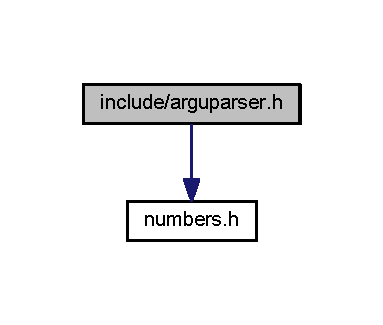
\includegraphics[width=184pt]{arguparser_8h__incl}
\end{center}
\end{figure}

\hypertarget{numbers_8h}{}\section{Référence du fichier include/numbers.h}
\label{numbers_8h}\index{include/numbers.\+h@{include/numbers.\+h}}


Toutes les fonctions en relation avec des nombres.  


Ce graphe montre quels fichiers incluent directement ou indirectement ce fichier \+:\nopagebreak
\begin{figure}[H]
\begin{center}
\leavevmode
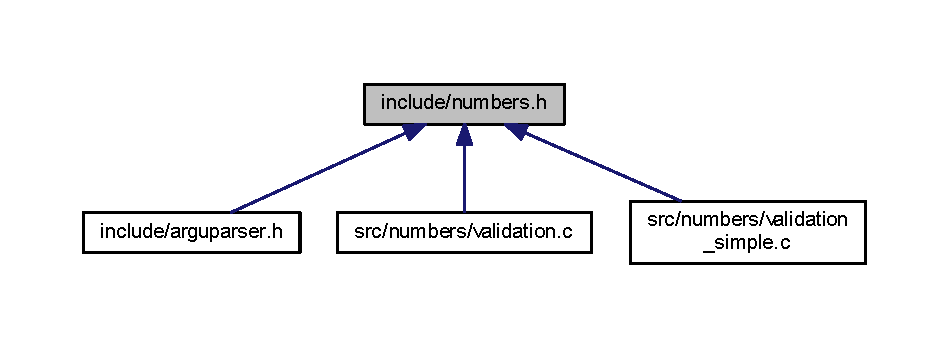
\includegraphics[width=350pt]{numbers_8h__dep__incl}
\end{center}
\end{figure}
\subsection*{Fonctions}
\begin{DoxyCompactItemize}
\item 
int \hyperlink{numbers_8h_ac6964a30af3665e1651e43b77d4ee261}{is\+\_\+valid\+\_\+nbr} (char $\ast$str, int $\ast$index)
\begin{DoxyCompactList}\small\item\em Vérifie si un entier naturel est valide. \end{DoxyCompactList}\item 
int \hyperlink{numbers_8h_a6992181d9ef9061cad273be1a264fe7e}{is\+\_\+valid\+\_\+float} (char $\ast$str, int $\ast$index)
\begin{DoxyCompactList}\small\item\em Vérifie si un nombre réel positif est valide. \end{DoxyCompactList}\item 
int \hyperlink{numbers_8h_a2f2beb5b51a2f859e0fb724833174fa3}{is\+\_\+valid\+\_\+signed} (char $\ast$str, int $\ast$index)
\begin{DoxyCompactList}\small\item\em Vérifie si un nombre entier est valide. \end{DoxyCompactList}\item 
int \hyperlink{numbers_8h_a20e05a6847277336ff170cbc5ff149d9}{is\+\_\+valid\+\_\+signedf} (char $\ast$str, int $\ast$index)
\begin{DoxyCompactList}\small\item\em Vérifie si un nombre réel est valide. \end{DoxyCompactList}\item 
int \hyperlink{numbers_8h_a319b8f80fc0eabc63c5d8a9566ce17eb}{is\+\_\+svalid\+\_\+nbr} (char $\ast$str)
\begin{DoxyCompactList}\small\item\em Vérifie si un entier naturel est valide. \end{DoxyCompactList}\item 
int \hyperlink{numbers_8h_a045b64c7d387939fb481485c012cdb46}{is\+\_\+svalid\+\_\+float} (char $\ast$str)
\begin{DoxyCompactList}\small\item\em Vérifie si un réel positif est valide. \end{DoxyCompactList}\item 
int \hyperlink{numbers_8h_a7ca01e23e4dc862cc69a2ca1213e7044}{is\+\_\+svalid\+\_\+signed} (char $\ast$str)
\begin{DoxyCompactList}\small\item\em Vérifie si un entier est valide. \end{DoxyCompactList}\item 
int \hyperlink{numbers_8h_a3816ca372248333aa48001f033151901}{is\+\_\+svalid\+\_\+signedf} (char $\ast$str)
\begin{DoxyCompactList}\small\item\em Vérifie si un réel est valide. \end{DoxyCompactList}\item 
int \hyperlink{numbers_8h_ae63e511d0f53ed0c5109ec858462f6b2}{is\+\_\+valid\+\_\+size} (char $\ast$str, int size)
\begin{DoxyCompactList}\small\item\em T\+O\+DO I do not know. \end{DoxyCompactList}\item 
int \hyperlink{numbers_8h_a8889d0ec835f57634693971aa2b01d01}{our\+\_\+stoi} (char $\ast$str)
\item 
long \hyperlink{numbers_8h_ae943c6a67c086512556a28a0be316ac3}{our\+\_\+stol} (char $\ast$str)
\item 
float \hyperlink{numbers_8h_a5d68c07a260f23bbf4320047ce0ccb4e}{our\+\_\+stof} (char $\ast$str)
\item 
double \hyperlink{numbers_8h_ab2d6e289191fd615337885f6f8f7a12a}{our\+\_\+stod} (char $\ast$str)
\end{DoxyCompactItemize}


\subsection{Description détaillée}
Toutes les fonctions en relation avec des nombres. 

Ce fichier rescence toutes les fonctions qui sont reliés aux nombres dans cette lib \begin{DoxySeeAlso}{Voir également}
../src/numbers/validation.c 

../src/numbers/validation\+\_\+simple.c 
\end{DoxySeeAlso}


\subsection{Documentation des fonctions}
\hypertarget{numbers_8h_a045b64c7d387939fb481485c012cdb46}{}\label{numbers_8h_a045b64c7d387939fb481485c012cdb46} 
\index{numbers.\+h@{numbers.\+h}!is\+\_\+svalid\+\_\+float@{is\+\_\+svalid\+\_\+float}}
\index{is\+\_\+svalid\+\_\+float@{is\+\_\+svalid\+\_\+float}!numbers.\+h@{numbers.\+h}}
\subsubsection{\texorpdfstring{is\+\_\+svalid\+\_\+float()}{is\_svalid\_float()}}
{\footnotesize\ttfamily int is\+\_\+svalid\+\_\+float (\begin{DoxyParamCaption}\item[{char $\ast$}]{str }\end{DoxyParamCaption})}



Vérifie si un réel positif est valide. 

Vérifie si le string donné contient un réel positif à partir du début jusqu\textquotesingle{}à la fin.


\begin{DoxyParams}{Paramètres}
{\em str} & La chaine de caractère à vérifier \\
\hline
\end{DoxyParams}


Définition à la ligne 18 du fichier validation\+\_\+simple.\+c.

\hypertarget{numbers_8h_a319b8f80fc0eabc63c5d8a9566ce17eb}{}\label{numbers_8h_a319b8f80fc0eabc63c5d8a9566ce17eb} 
\index{numbers.\+h@{numbers.\+h}!is\+\_\+svalid\+\_\+nbr@{is\+\_\+svalid\+\_\+nbr}}
\index{is\+\_\+svalid\+\_\+nbr@{is\+\_\+svalid\+\_\+nbr}!numbers.\+h@{numbers.\+h}}
\subsubsection{\texorpdfstring{is\+\_\+svalid\+\_\+nbr()}{is\_svalid\_nbr()}}
{\footnotesize\ttfamily int is\+\_\+svalid\+\_\+nbr (\begin{DoxyParamCaption}\item[{char $\ast$}]{str }\end{DoxyParamCaption})}



Vérifie si un entier naturel est valide. 

Vérifie si le string donné contient un entier naturel à partir du début jusqu\textquotesingle{}à la fin.


\begin{DoxyParams}{Paramètres}
{\em str} & La chaine de caractère à vérifier \\
\hline
\end{DoxyParams}


Définition à la ligne 10 du fichier validation\+\_\+simple.\+c.

\hypertarget{numbers_8h_a7ca01e23e4dc862cc69a2ca1213e7044}{}\label{numbers_8h_a7ca01e23e4dc862cc69a2ca1213e7044} 
\index{numbers.\+h@{numbers.\+h}!is\+\_\+svalid\+\_\+signed@{is\+\_\+svalid\+\_\+signed}}
\index{is\+\_\+svalid\+\_\+signed@{is\+\_\+svalid\+\_\+signed}!numbers.\+h@{numbers.\+h}}
\subsubsection{\texorpdfstring{is\+\_\+svalid\+\_\+signed()}{is\_svalid\_signed()}}
{\footnotesize\ttfamily int is\+\_\+svalid\+\_\+signed (\begin{DoxyParamCaption}\item[{char $\ast$}]{str }\end{DoxyParamCaption})}



Vérifie si un entier est valide. 

Check if the number is valid as signed from the beginning to the end


\begin{DoxyParams}{Paramètres}
{\em str} & La chaine de caractère à vérifier \\
\hline
\end{DoxyParams}


Définition à la ligne 26 du fichier validation\+\_\+simple.\+c.

\hypertarget{numbers_8h_a3816ca372248333aa48001f033151901}{}\label{numbers_8h_a3816ca372248333aa48001f033151901} 
\index{numbers.\+h@{numbers.\+h}!is\+\_\+svalid\+\_\+signedf@{is\+\_\+svalid\+\_\+signedf}}
\index{is\+\_\+svalid\+\_\+signedf@{is\+\_\+svalid\+\_\+signedf}!numbers.\+h@{numbers.\+h}}
\subsubsection{\texorpdfstring{is\+\_\+svalid\+\_\+signedf()}{is\_svalid\_signedf()}}
{\footnotesize\ttfamily int is\+\_\+svalid\+\_\+signedf (\begin{DoxyParamCaption}\item[{char $\ast$}]{str }\end{DoxyParamCaption})}



Vérifie si un réel est valide. 

Vérifie si le string donné contient un réel à partir du début jusqu\textquotesingle{}à la fin.


\begin{DoxyParams}{Paramètres}
{\em str} & La chaine de caractère à vérifier \\
\hline
\end{DoxyParams}


Définition à la ligne 34 du fichier validation\+\_\+simple.\+c.

\hypertarget{numbers_8h_a6992181d9ef9061cad273be1a264fe7e}{}\label{numbers_8h_a6992181d9ef9061cad273be1a264fe7e} 
\index{numbers.\+h@{numbers.\+h}!is\+\_\+valid\+\_\+float@{is\+\_\+valid\+\_\+float}}
\index{is\+\_\+valid\+\_\+float@{is\+\_\+valid\+\_\+float}!numbers.\+h@{numbers.\+h}}
\subsubsection{\texorpdfstring{is\+\_\+valid\+\_\+float()}{is\_valid\_float()}}
{\footnotesize\ttfamily int is\+\_\+valid\+\_\+float (\begin{DoxyParamCaption}\item[{char $\ast$}]{str,  }\item[{int $\ast$}]{index }\end{DoxyParamCaption})}



Vérifie si un nombre réel positif est valide. 

Vérifie si le string donné contient un réel positif à partir de \textquotesingle{}index\textquotesingle{} jusqu\textquotesingle{}à la fin.


\begin{DoxyParams}{Paramètres}
{\em str} & La chaine de caractère à vérifier \\
\hline
{\em index} & L\textquotesingle{}index de départ \\
\hline
\end{DoxyParams}


Définition à la ligne 23 du fichier validation.\+c.

\hypertarget{numbers_8h_ac6964a30af3665e1651e43b77d4ee261}{}\label{numbers_8h_ac6964a30af3665e1651e43b77d4ee261} 
\index{numbers.\+h@{numbers.\+h}!is\+\_\+valid\+\_\+nbr@{is\+\_\+valid\+\_\+nbr}}
\index{is\+\_\+valid\+\_\+nbr@{is\+\_\+valid\+\_\+nbr}!numbers.\+h@{numbers.\+h}}
\subsubsection{\texorpdfstring{is\+\_\+valid\+\_\+nbr()}{is\_valid\_nbr()}}
{\footnotesize\ttfamily int is\+\_\+valid\+\_\+nbr (\begin{DoxyParamCaption}\item[{char $\ast$}]{str,  }\item[{int $\ast$}]{index }\end{DoxyParamCaption})}



Vérifie si un entier naturel est valide. 

Vérifie si le string donné contient un entier naturel à partir de \textquotesingle{}index\textquotesingle{} jusqu\textquotesingle{}à la fin.


\begin{DoxyParams}{Paramètres}
{\em str} & La chaine de caractère à vérifier \\
\hline
{\em index} & L\textquotesingle{}index de départ \\
\hline
\end{DoxyParams}


Définition à la ligne 10 du fichier validation.\+c.

\hypertarget{numbers_8h_a2f2beb5b51a2f859e0fb724833174fa3}{}\label{numbers_8h_a2f2beb5b51a2f859e0fb724833174fa3} 
\index{numbers.\+h@{numbers.\+h}!is\+\_\+valid\+\_\+signed@{is\+\_\+valid\+\_\+signed}}
\index{is\+\_\+valid\+\_\+signed@{is\+\_\+valid\+\_\+signed}!numbers.\+h@{numbers.\+h}}
\subsubsection{\texorpdfstring{is\+\_\+valid\+\_\+signed()}{is\_valid\_signed()}}
{\footnotesize\ttfamily int is\+\_\+valid\+\_\+signed (\begin{DoxyParamCaption}\item[{char $\ast$}]{str,  }\item[{int $\ast$}]{index }\end{DoxyParamCaption})}



Vérifie si un nombre entier est valide. 

Vérifie si le string donné contient un entier à partir de \textquotesingle{}index\textquotesingle{} jusqu\textquotesingle{}à la fin.


\begin{DoxyParams}{Paramètres}
{\em str} & La chaine de caractère à vérifier \\
\hline
{\em index} & L\textquotesingle{}index de départ \\
\hline
\end{DoxyParams}


Définition à la ligne 37 du fichier validation.\+c.

\hypertarget{numbers_8h_a20e05a6847277336ff170cbc5ff149d9}{}\label{numbers_8h_a20e05a6847277336ff170cbc5ff149d9} 
\index{numbers.\+h@{numbers.\+h}!is\+\_\+valid\+\_\+signedf@{is\+\_\+valid\+\_\+signedf}}
\index{is\+\_\+valid\+\_\+signedf@{is\+\_\+valid\+\_\+signedf}!numbers.\+h@{numbers.\+h}}
\subsubsection{\texorpdfstring{is\+\_\+valid\+\_\+signedf()}{is\_valid\_signedf()}}
{\footnotesize\ttfamily int is\+\_\+valid\+\_\+signedf (\begin{DoxyParamCaption}\item[{char $\ast$}]{str,  }\item[{int $\ast$}]{index }\end{DoxyParamCaption})}



Vérifie si un nombre réel est valide. 

Vérifie si le string donné contient un réel à partir de \textquotesingle{}index\textquotesingle{} jusqu\textquotesingle{}à la fin.


\begin{DoxyParams}{Paramètres}
{\em str} & La chaine de caractère à vérifier \\
\hline
{\em index} & L\textquotesingle{}index de départ \\
\hline
\end{DoxyParams}


Définition à la ligne 46 du fichier validation.\+c.

\hypertarget{numbers_8h_ae63e511d0f53ed0c5109ec858462f6b2}{}\label{numbers_8h_ae63e511d0f53ed0c5109ec858462f6b2} 
\index{numbers.\+h@{numbers.\+h}!is\+\_\+valid\+\_\+size@{is\+\_\+valid\+\_\+size}}
\index{is\+\_\+valid\+\_\+size@{is\+\_\+valid\+\_\+size}!numbers.\+h@{numbers.\+h}}
\subsubsection{\texorpdfstring{is\+\_\+valid\+\_\+size()}{is\_valid\_size()}}
{\footnotesize\ttfamily int is\+\_\+valid\+\_\+size (\begin{DoxyParamCaption}\item[{char $\ast$}]{str,  }\item[{int}]{size }\end{DoxyParamCaption})}



T\+O\+DO I do not know. 

\hypertarget{numbers_8h_ab2d6e289191fd615337885f6f8f7a12a}{}\label{numbers_8h_ab2d6e289191fd615337885f6f8f7a12a} 
\index{numbers.\+h@{numbers.\+h}!our\+\_\+stod@{our\+\_\+stod}}
\index{our\+\_\+stod@{our\+\_\+stod}!numbers.\+h@{numbers.\+h}}
\subsubsection{\texorpdfstring{our\+\_\+stod()}{our\_stod()}}
{\footnotesize\ttfamily double our\+\_\+stod (\begin{DoxyParamCaption}\item[{char $\ast$}]{str }\end{DoxyParamCaption})}

\hypertarget{numbers_8h_a5d68c07a260f23bbf4320047ce0ccb4e}{}\label{numbers_8h_a5d68c07a260f23bbf4320047ce0ccb4e} 
\index{numbers.\+h@{numbers.\+h}!our\+\_\+stof@{our\+\_\+stof}}
\index{our\+\_\+stof@{our\+\_\+stof}!numbers.\+h@{numbers.\+h}}
\subsubsection{\texorpdfstring{our\+\_\+stof()}{our\_stof()}}
{\footnotesize\ttfamily float our\+\_\+stof (\begin{DoxyParamCaption}\item[{char $\ast$}]{str }\end{DoxyParamCaption})}

\hypertarget{numbers_8h_a8889d0ec835f57634693971aa2b01d01}{}\label{numbers_8h_a8889d0ec835f57634693971aa2b01d01} 
\index{numbers.\+h@{numbers.\+h}!our\+\_\+stoi@{our\+\_\+stoi}}
\index{our\+\_\+stoi@{our\+\_\+stoi}!numbers.\+h@{numbers.\+h}}
\subsubsection{\texorpdfstring{our\+\_\+stoi()}{our\_stoi()}}
{\footnotesize\ttfamily int our\+\_\+stoi (\begin{DoxyParamCaption}\item[{char $\ast$}]{str }\end{DoxyParamCaption})}

\hypertarget{numbers_8h_ae943c6a67c086512556a28a0be316ac3}{}\label{numbers_8h_ae943c6a67c086512556a28a0be316ac3} 
\index{numbers.\+h@{numbers.\+h}!our\+\_\+stol@{our\+\_\+stol}}
\index{our\+\_\+stol@{our\+\_\+stol}!numbers.\+h@{numbers.\+h}}
\subsubsection{\texorpdfstring{our\+\_\+stol()}{our\_stol()}}
{\footnotesize\ttfamily long our\+\_\+stol (\begin{DoxyParamCaption}\item[{char $\ast$}]{str }\end{DoxyParamCaption})}


\hypertarget{validation_8c}{}\section{Référence du fichier src/numbers/validation.c}
\label{validation_8c}\index{src/numbers/validation.\+c@{src/numbers/validation.\+c}}


Déclaration des fonctions de validation.  


{\ttfamily \#include \char`\"{}../../include/numbers.\+h\char`\"{}}\newline
Graphe des dépendances par inclusion de validation.\+c\+:\nopagebreak
\begin{figure}[H]
\begin{center}
\leavevmode
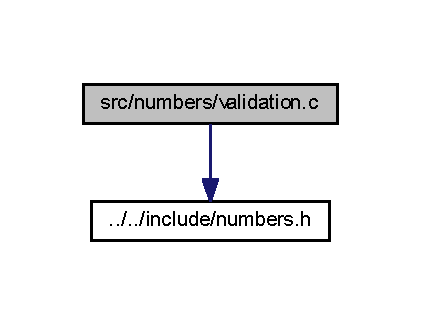
\includegraphics[width=202pt]{validation_8c__incl}
\end{center}
\end{figure}
\subsection*{Fonctions}
\begin{DoxyCompactItemize}
\item 
int \hyperlink{validation_8c_ac6964a30af3665e1651e43b77d4ee261}{is\+\_\+valid\+\_\+nbr} (char $\ast$str, int $\ast$index)
\begin{DoxyCompactList}\small\item\em Vérifie si un entier naturel est valide. \end{DoxyCompactList}\item 
int \hyperlink{validation_8c_a6992181d9ef9061cad273be1a264fe7e}{is\+\_\+valid\+\_\+float} (char $\ast$str, int $\ast$index)
\begin{DoxyCompactList}\small\item\em Vérifie si un nombre réel positif est valide. \end{DoxyCompactList}\item 
int \hyperlink{validation_8c_a2f2beb5b51a2f859e0fb724833174fa3}{is\+\_\+valid\+\_\+signed} (char $\ast$str, int $\ast$index)
\begin{DoxyCompactList}\small\item\em Vérifie si un nombre entier est valide. \end{DoxyCompactList}\item 
int \hyperlink{validation_8c_a20e05a6847277336ff170cbc5ff149d9}{is\+\_\+valid\+\_\+signedf} (char $\ast$str, int $\ast$index)
\begin{DoxyCompactList}\small\item\em Vérifie si un nombre réel est valide. \end{DoxyCompactList}\end{DoxyCompactItemize}


\subsection{Description détaillée}
Déclaration des fonctions de validation. 

Déclaration des fonctions complètes de validation des nombres 

\subsection{Documentation des fonctions}
\hypertarget{validation_8c_a6992181d9ef9061cad273be1a264fe7e}{}\label{validation_8c_a6992181d9ef9061cad273be1a264fe7e} 
\index{validation.\+c@{validation.\+c}!is\+\_\+valid\+\_\+float@{is\+\_\+valid\+\_\+float}}
\index{is\+\_\+valid\+\_\+float@{is\+\_\+valid\+\_\+float}!validation.\+c@{validation.\+c}}
\subsubsection{\texorpdfstring{is\+\_\+valid\+\_\+float()}{is\_valid\_float()}}
{\footnotesize\ttfamily int is\+\_\+valid\+\_\+float (\begin{DoxyParamCaption}\item[{char $\ast$}]{str,  }\item[{int $\ast$}]{index }\end{DoxyParamCaption})}



Vérifie si un nombre réel positif est valide. 

Vérifie si le string donné contient un réel positif à partir de \textquotesingle{}index\textquotesingle{} jusqu\textquotesingle{}à la fin.


\begin{DoxyParams}{Paramètres}
{\em str} & La chaine de caractère à vérifier \\
\hline
{\em index} & L\textquotesingle{}index de départ \\
\hline
\end{DoxyParams}


Définition à la ligne 23 du fichier validation.\+c.

\hypertarget{validation_8c_ac6964a30af3665e1651e43b77d4ee261}{}\label{validation_8c_ac6964a30af3665e1651e43b77d4ee261} 
\index{validation.\+c@{validation.\+c}!is\+\_\+valid\+\_\+nbr@{is\+\_\+valid\+\_\+nbr}}
\index{is\+\_\+valid\+\_\+nbr@{is\+\_\+valid\+\_\+nbr}!validation.\+c@{validation.\+c}}
\subsubsection{\texorpdfstring{is\+\_\+valid\+\_\+nbr()}{is\_valid\_nbr()}}
{\footnotesize\ttfamily int is\+\_\+valid\+\_\+nbr (\begin{DoxyParamCaption}\item[{char $\ast$}]{str,  }\item[{int $\ast$}]{index }\end{DoxyParamCaption})}



Vérifie si un entier naturel est valide. 

Vérifie si le string donné contient un entier naturel à partir de \textquotesingle{}index\textquotesingle{} jusqu\textquotesingle{}à la fin.


\begin{DoxyParams}{Paramètres}
{\em str} & La chaine de caractère à vérifier \\
\hline
{\em index} & L\textquotesingle{}index de départ \\
\hline
\end{DoxyParams}


Définition à la ligne 10 du fichier validation.\+c.

\hypertarget{validation_8c_a2f2beb5b51a2f859e0fb724833174fa3}{}\label{validation_8c_a2f2beb5b51a2f859e0fb724833174fa3} 
\index{validation.\+c@{validation.\+c}!is\+\_\+valid\+\_\+signed@{is\+\_\+valid\+\_\+signed}}
\index{is\+\_\+valid\+\_\+signed@{is\+\_\+valid\+\_\+signed}!validation.\+c@{validation.\+c}}
\subsubsection{\texorpdfstring{is\+\_\+valid\+\_\+signed()}{is\_valid\_signed()}}
{\footnotesize\ttfamily int is\+\_\+valid\+\_\+signed (\begin{DoxyParamCaption}\item[{char $\ast$}]{str,  }\item[{int $\ast$}]{index }\end{DoxyParamCaption})}



Vérifie si un nombre entier est valide. 

Vérifie si le string donné contient un entier à partir de \textquotesingle{}index\textquotesingle{} jusqu\textquotesingle{}à la fin.


\begin{DoxyParams}{Paramètres}
{\em str} & La chaine de caractère à vérifier \\
\hline
{\em index} & L\textquotesingle{}index de départ \\
\hline
\end{DoxyParams}


Définition à la ligne 37 du fichier validation.\+c.

\hypertarget{validation_8c_a20e05a6847277336ff170cbc5ff149d9}{}\label{validation_8c_a20e05a6847277336ff170cbc5ff149d9} 
\index{validation.\+c@{validation.\+c}!is\+\_\+valid\+\_\+signedf@{is\+\_\+valid\+\_\+signedf}}
\index{is\+\_\+valid\+\_\+signedf@{is\+\_\+valid\+\_\+signedf}!validation.\+c@{validation.\+c}}
\subsubsection{\texorpdfstring{is\+\_\+valid\+\_\+signedf()}{is\_valid\_signedf()}}
{\footnotesize\ttfamily int is\+\_\+valid\+\_\+signedf (\begin{DoxyParamCaption}\item[{char $\ast$}]{str,  }\item[{int $\ast$}]{index }\end{DoxyParamCaption})}



Vérifie si un nombre réel est valide. 

Vérifie si le string donné contient un réel à partir de \textquotesingle{}index\textquotesingle{} jusqu\textquotesingle{}à la fin.


\begin{DoxyParams}{Paramètres}
{\em str} & La chaine de caractère à vérifier \\
\hline
{\em index} & L\textquotesingle{}index de départ \\
\hline
\end{DoxyParams}


Définition à la ligne 46 du fichier validation.\+c.


\hypertarget{validation__simple_8c}{}\section{Référence du fichier src/numbers/validation\+\_\+simple.c}
\label{validation__simple_8c}\index{src/numbers/validation\+\_\+simple.\+c@{src/numbers/validation\+\_\+simple.\+c}}


Déclaration des fonctions de validation.  


{\ttfamily \#include \char`\"{}../../include/numbers.\+h\char`\"{}}\newline
Graphe des dépendances par inclusion de validation\+\_\+simple.\+c\+:\nopagebreak
\begin{figure}[H]
\begin{center}
\leavevmode
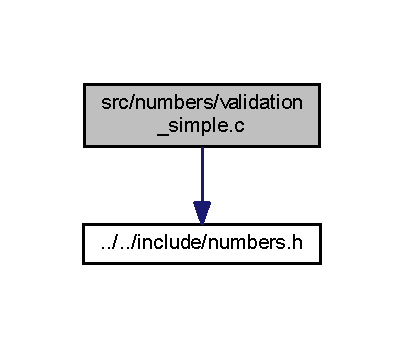
\includegraphics[width=194pt]{validation__simple_8c__incl}
\end{center}
\end{figure}
\subsection*{Fonctions}
\begin{DoxyCompactItemize}
\item 
int \hyperlink{validation__simple_8c_a319b8f80fc0eabc63c5d8a9566ce17eb}{is\+\_\+svalid\+\_\+nbr} (char $\ast$str)
\begin{DoxyCompactList}\small\item\em Vérifie si un entier naturel est valide. \end{DoxyCompactList}\item 
int \hyperlink{validation__simple_8c_a045b64c7d387939fb481485c012cdb46}{is\+\_\+svalid\+\_\+float} (char $\ast$str)
\begin{DoxyCompactList}\small\item\em Vérifie si un réel positif est valide. \end{DoxyCompactList}\item 
int \hyperlink{validation__simple_8c_a7ca01e23e4dc862cc69a2ca1213e7044}{is\+\_\+svalid\+\_\+signed} (char $\ast$str)
\begin{DoxyCompactList}\small\item\em Vérifie si un entier est valide. \end{DoxyCompactList}\item 
int \hyperlink{validation__simple_8c_a3816ca372248333aa48001f033151901}{is\+\_\+svalid\+\_\+signedf} (char $\ast$str)
\begin{DoxyCompactList}\small\item\em Vérifie si un réel est valide. \end{DoxyCompactList}\end{DoxyCompactItemize}


\subsection{Description détaillée}
Déclaration des fonctions de validation. 

Déclaration des fonctions simplifiés de validation des nombres 

\subsection{Documentation des fonctions}
\hypertarget{validation__simple_8c_a045b64c7d387939fb481485c012cdb46}{}\label{validation__simple_8c_a045b64c7d387939fb481485c012cdb46} 
\index{validation\+\_\+simple.\+c@{validation\+\_\+simple.\+c}!is\+\_\+svalid\+\_\+float@{is\+\_\+svalid\+\_\+float}}
\index{is\+\_\+svalid\+\_\+float@{is\+\_\+svalid\+\_\+float}!validation\+\_\+simple.\+c@{validation\+\_\+simple.\+c}}
\subsubsection{\texorpdfstring{is\+\_\+svalid\+\_\+float()}{is\_svalid\_float()}}
{\footnotesize\ttfamily int is\+\_\+svalid\+\_\+float (\begin{DoxyParamCaption}\item[{char $\ast$}]{str }\end{DoxyParamCaption})}



Vérifie si un réel positif est valide. 

Vérifie si le string donné contient un réel positif à partir du début jusqu\textquotesingle{}à la fin.


\begin{DoxyParams}{Paramètres}
{\em str} & La chaine de caractère à vérifier \\
\hline
\end{DoxyParams}


Définition à la ligne 18 du fichier validation\+\_\+simple.\+c.

\hypertarget{validation__simple_8c_a319b8f80fc0eabc63c5d8a9566ce17eb}{}\label{validation__simple_8c_a319b8f80fc0eabc63c5d8a9566ce17eb} 
\index{validation\+\_\+simple.\+c@{validation\+\_\+simple.\+c}!is\+\_\+svalid\+\_\+nbr@{is\+\_\+svalid\+\_\+nbr}}
\index{is\+\_\+svalid\+\_\+nbr@{is\+\_\+svalid\+\_\+nbr}!validation\+\_\+simple.\+c@{validation\+\_\+simple.\+c}}
\subsubsection{\texorpdfstring{is\+\_\+svalid\+\_\+nbr()}{is\_svalid\_nbr()}}
{\footnotesize\ttfamily int is\+\_\+svalid\+\_\+nbr (\begin{DoxyParamCaption}\item[{char $\ast$}]{str }\end{DoxyParamCaption})}



Vérifie si un entier naturel est valide. 

Vérifie si le string donné contient un entier naturel à partir du début jusqu\textquotesingle{}à la fin.


\begin{DoxyParams}{Paramètres}
{\em str} & La chaine de caractère à vérifier \\
\hline
\end{DoxyParams}


Définition à la ligne 10 du fichier validation\+\_\+simple.\+c.

\hypertarget{validation__simple_8c_a7ca01e23e4dc862cc69a2ca1213e7044}{}\label{validation__simple_8c_a7ca01e23e4dc862cc69a2ca1213e7044} 
\index{validation\+\_\+simple.\+c@{validation\+\_\+simple.\+c}!is\+\_\+svalid\+\_\+signed@{is\+\_\+svalid\+\_\+signed}}
\index{is\+\_\+svalid\+\_\+signed@{is\+\_\+svalid\+\_\+signed}!validation\+\_\+simple.\+c@{validation\+\_\+simple.\+c}}
\subsubsection{\texorpdfstring{is\+\_\+svalid\+\_\+signed()}{is\_svalid\_signed()}}
{\footnotesize\ttfamily int is\+\_\+svalid\+\_\+signed (\begin{DoxyParamCaption}\item[{char $\ast$}]{str }\end{DoxyParamCaption})}



Vérifie si un entier est valide. 

Check if the number is valid as signed from the beginning to the end


\begin{DoxyParams}{Paramètres}
{\em str} & La chaine de caractère à vérifier \\
\hline
\end{DoxyParams}


Définition à la ligne 26 du fichier validation\+\_\+simple.\+c.

\hypertarget{validation__simple_8c_a3816ca372248333aa48001f033151901}{}\label{validation__simple_8c_a3816ca372248333aa48001f033151901} 
\index{validation\+\_\+simple.\+c@{validation\+\_\+simple.\+c}!is\+\_\+svalid\+\_\+signedf@{is\+\_\+svalid\+\_\+signedf}}
\index{is\+\_\+svalid\+\_\+signedf@{is\+\_\+svalid\+\_\+signedf}!validation\+\_\+simple.\+c@{validation\+\_\+simple.\+c}}
\subsubsection{\texorpdfstring{is\+\_\+svalid\+\_\+signedf()}{is\_svalid\_signedf()}}
{\footnotesize\ttfamily int is\+\_\+svalid\+\_\+signedf (\begin{DoxyParamCaption}\item[{char $\ast$}]{str }\end{DoxyParamCaption})}



Vérifie si un réel est valide. 

Vérifie si le string donné contient un réel à partir du début jusqu\textquotesingle{}à la fin.


\begin{DoxyParams}{Paramètres}
{\em str} & La chaine de caractère à vérifier \\
\hline
\end{DoxyParams}


Définition à la ligne 34 du fichier validation\+\_\+simple.\+c.


%--- End generated contents ---

% Index
\backmatter
\newpage
\phantomsection
\clearemptydoublepage
\addcontentsline{toc}{chapter}{Index}
\printindex

\end{document}
